\documentclass[10pt]{article}
\usepackage[utf8]{inputenc}
\usepackage[spanish, activeacute]{babel}
\usepackage{amsmath}
\usepackage{epsfig}
\usepackage{enumerate}
\usepackage{float}
\usepackage{listings}
\frenchspacing
\linespread{1.2}                                          %espacio entre líneas
\setlength{\parskip}{1.5ex plus 0.2ex minus 0.2ex}        %espacio entre párrafos
\setlength{\columnsep}{0.9cm}  				  %espacio entre columnas
\usepackage{indentfirst}
\usepackage{graphicx}
\usepackage{verbatim}
\usepackage{url}
\usepackage{multicol}
\usepackage{geometry}
\usepackage{fancyhdr}
\usepackage{moreverb}
\usepackage{hyperref}
\usepackage{acronym}

\geometry{tmargin=3.0cm, lmargin=3.0cm, rmargin=2.5cm, bmargin=3.0cm}

\newcommand\R{R}
\newenvironment{keywords}{\begin{description}\item[Palabras Claves:]}{\end{description}}
\renewcommand{\refname}{Referencias}

\title{
\center{\emph{Desarrollo de una plataforma astroinformática para la administración y análisis inteligente de datos a gran escala} \\}
\center{\textbf{Arquitectura de software - Prototipo Funcional 
	\\ Version 1.3 - 26 Diciembre} \\}
\author{Mauricio Solar, Marcelo Mendoza, Diego Mardones, Jonathan Antognini, \\ 
	Walter Fariña, Christopher Fernandez, Mario Garces, \\	
	Camilo Valenzuela, Patricio Ramirez, Marco Peña.}
\date{Valparaíso, \today}
}

\begin{document}
\maketitle

\thispagestyle{empty}

\newpage
\tableofcontents

\newpage
\section{Indice de acrónimos}
\begin{acronym}
\acro{ChiVO}{Chilean Virtual Observatory}
\acro{VO}{Virtual Observatory}
\acro{ALMA}{Atacama Large Milimiter/submilimiter Array}
\acro{UV}{Ultravioleta}
\acro{FITS}{Flexible Image Transport System}
\acro{ASDM}{ALMA Science Data Model}
\acro{J2000}{Fecha Juliana 2451545.0 Tiempo Terrestre. Es equivalente al 1 de
enero de 2000, 11:59:27.816. Se usa para indicar un instante en el tiempo
estándar para la medición de las posiciones de los cuerpos celestes y otros
eventos estelares}
\acro{B1950}{Época besseliana, es una época basada en el Año besseliano, que es
un año tropical medido en el punto donde la longitud del Sol es exactamente
280º}
\acro{Sesame}{Es un resolvedor de nombres que retorna a partir de una cadena
que representa la designación de un objeto astronómico fuera del Sistema Solar,
la posición del objeto en el cielo y otros detalles}
\acro{SIMBAD}{Base de datos que proporciona datos básicos, identificaciones
cruzadas, bibliografía y las mediciones de los objetos astronómicos fuera del
sistema solar.}
\acro{ADS}{Astrophysics Data System, es una librería/portal digital}
\acro{NED}{SA/IPAC Extragalactic Database, ofrece datos de millones de objetos
fuera de la Vía Láctea.}
\acro{IVOA}{International Virtual Observatory Alliance}
\acro{SCS}{Simple Cone Search}
\acro{SIA}{Simple Image Access}
\acro{SSA}{Simple Spectral Access}
\acro{TAP}{Table Access Protocol}
\acro{MQ}{Message Queuing}
\end{acronym}


\newpage
\section{Resumen Ejecutivo}


\newpage
\section{Casos de Uso ChiVO}
\noindent En la captura de requerimientos y casos de uso participaron los siguientes
astrónomos:
\begin{itemize}
	\item Diego Mardones, Universidad de Chile.
	\item Lars Nyman, Atacama Large Milimiter/submilimiter Array.
	\item Neil Nagar, Universidad de Concepción.
	\item Nelson Padilla, Pontificie Universidad Católica. 
	\item Juan de Santander, Instituto de Astrofísica de Andalucía, España.
	\item Amelia Bayo, European Southern Observatory.
\end{itemize}

\noindent El informe de requerimientos (Hito Anterior) se puede encontrar en
\cite{hrequerimientos}.

\noindent Para abordar de mejor forma los casos de uso, se mencionarán algunos
conceptos relevantes:
\begin{itemize}
	\item Los datos astronómicos en sus diferentes formatos se dividen en:
Metadata y Binarios. La metadata son datos que describen los datos de la
observación, y los binarios son los datos obtenidos de la observación.
	\item En la primera etapa el proyecto trabajará con archivos FITS.
	\item Las búsquedas en el sistema se realizan sobre la metadata. El
resultado de una búsqueda es un set de datos candidatos que coinciden con los
parámetros fijados en la búsqueda.
	\item La interacción final con el sistema es cuando el usuario decide qué
datos necesita, los selecciona y los descarga de forma local.
\end{itemize}

\subsection{Casos de Uso Generales}
Los siguientes casos de usos involucran de manera general a varios
requerimientos, por lo que se presentan en una categoría especial. 

\noindent\textbf{Caso de uso \#1}: \\
\textbf{Objetivo}: Filtrar los resultados de la búsqueda en el Portal Web. \\
\textbf{Actor}: Usuario. \\
\textbf{Necesidad}: Esencial. \\
\textbf{Prioridad}: Alta. \\
\textbf{Requerimientos Referenciados}: del 1 al 7. \\
\textbf{Descripción}: Ya que el usuario puede recibir una gran cantidad de
resultados, éste debe ser capaz de realizar un filtro sobre alguna columna de
los datos recibidos al realizar la búsqueda para así poder identificar los
datos que se encuentre buscando. Este filtro puede ser realizado en el mismo
navegador del usuario o a través de una nueva consulta. 
\vspace{1.0cm}

\noindent\textbf{Caso de uso \#2}: \\
\textbf{Objetivo}: Descargar datos desde el Portal Web. \\
\textbf{Actor}: Usuario. \\
\textbf{Necesidad}: Esencial. \\
\textbf{Prioridad}: Alta. \\
\textbf{Requerimientos Referenciados}: del 1 al 7. \\
\textbf{Descripción}: Una vez que el usuario encuentre los datos que requiere, éste procede a descargarlos. Para ello el sistema provee un enlace directo a la fuente de los datos.
\vspace{1.0cm}

\noindent\textbf{Caso de uso \#3}: \\
\textbf{Objetivo}: Visualizar una representación gráfica que compare los metadatos de los resultados de la búsqueda. \\
\textbf{Actor}: Usuario. \\
\textbf{Necesidad}: Esencial. \\
\textbf{Prioridad}:  Media. \\
\textbf{Requerimientos Referenciados}: del 1 al 7. \\
\textbf{Descripción}: Una vez que el usuario reciba un conjunto de resultados, podrá visualizarlos en gráficos acordes al tipo de búsqueda y en base a los metadatos recibidos por la búsqueda.
\vspace{1.0cm}

\noindent\textbf{Caso de uso \#4}: \\
\textbf{Objetivo}: Visualizar un producto o subproducto de los datos de la observación presente en los metadatos. \\
\textbf{Actor}: Usuario. \\
\textbf{Necesidad}: Esencial. \\
\textbf{Prioridad}: Alta. \\
\textbf{Requerimientos Referenciados}: del 1 al 7. \\
\textbf{Descripción}: Visualización de la forma geométrica de las observaciones (rectangulares o redondas); cobertura UV; Calibración de paso de banda;Espectro observado;Imagen observada en un plano del producto cuando sea posible (podría ser parte de análisis en vez de observación);
\vspace{1.0cm}

\noindent\textbf{Caso de uso \#5}: \\
\textbf{Objetivo}: Análisis de cubo FITS. \\
\textbf{Actor}: Usuario.\\
\textbf{Necesidad}: Esencial. \\
\textbf{Prioridad}: Alta. \\
\textbf{Requerimientos Referenciados}: del 1 al 7. \\
\textbf{Descripción}: Selecciona pixeles; proyección en una dimensión;flujo en un área;series de tiempo.
\vspace{1.0cm}

\noindent\textbf{Caso de uso \#6}: \\
\textbf{Objetivo}: Análisis de ASDM. \\
\textbf{Actor}: Usuario. \\
\textbf{Necesidad}: Deseable. \\
\textbf{Prioridad}: Media. \\
\textbf{Requerimientos Referenciados}: del 1 al 7. \\
\textbf{Descripción}: Selecciona voxeles; proyección en una dimensión;flujo en un área;series de tiempo.
\vspace{1.0cm}

\noindent\textbf{Caso de uso \#7}: \\
\textbf{Objetivo}: Los resultados de la búsqueda deben ser analizables para secuencias de tiempo. \\
\textbf{Actor}: Usuario. \\
\textbf{Necesidad}: Esencial. \\
\textbf{Prioridad}: Baja. \\
\textbf{Requerimientos Referenciados}: del 1 al 7. \\
\textbf{Descripción}: El usuario luego de realizar una búsqueda por tipo y/o subtipo de objeto, puede obtener los resultados de la búsqueda para ser analizados como secuencias de tiempo.
\vspace{1.0cm}

\subsection{Buscar por coordenada o región del cielo}
\noindent\textbf{Caso de uso \#8}: \\
\textbf{Objetivo}: Ingresar al Portal Web y realizar una búsqueda por coordenadas. \\
\textbf{Actor}: Usuario. \\
\textbf{Necesidad}: Esencial. \\
\textbf{Prioridad}: Alta. \\
\textbf{Requerimientos Referenciados}: 1. \\
\textbf{Descripción}: El usuario ingresa al Portal Web, rellena los campos de coordenadas y radio angular o región de cielo y realiza una búsqueda. Los parámetros de coordenada pueden pertenecer al sistema ecuatorial (J2000 o B1950), eclíptico, galáctico o supergaláctico.
\vspace{1.0cm}

\noindent\textbf{Caso de uso \#9}: \\
\textbf{Objetivo}: Realizar una búsqueda de listado de coordenadas. \\
\textbf{Actor}: Usuario. \\
\textbf{Necesidad}: Esencial. \\
\textbf{Prioridad}: Alta. \\
\textbf{Requerimientos Referenciados}: 1. \\
\textbf{Descripción}: El usuario ingresa al Portal Web, ingresa una lista de coordenadas y radios angulares o regiones de cielo y realiza una búsqueda. Los parámetros de coordenada pueden pertenecer al sistema ecuatorial (J2000 o B1950), eclíptico, galáctico o supergaláctico. También el usuario puede subir un archivo con un formato establecido por el sitio con el listado de coordenadas.
\vspace{1.0cm}

\subsection{Buscar por nombre o tipo de objeto}
\textbf{Caso de uso \#10}: \\
\noindent\textbf{Objetivo}: Ingresar al Portal Web y realizar una búsqueda por nombre en base a Sesame. \\
\textbf{Actor}: Usuario.\\
\textbf{Necesidad}: Esencial.\\
\textbf{Prioridad}: Alta.\\
\textbf{Requerimientos Referenciados}: 2. \\
\textbf{Descripción}: El usuario ingresa al Portal Web, rellena el campo de nombre según los nombres definidos en Sesame y realiza una búsqueda.
\vspace{1.0cm}

\noindent\textbf{Caso de uso \#11}: \\
\textbf{Objetivo}: Ingresar al Portal Web y realizar una búsqueda por nombre en base a catálogo de un instrumento. \\
\textbf{Actor}: Usuario.\\
\textbf{Necesidad}: Esencial.\\
\textbf{Prioridad}: Alta.\\
\textbf{Requerimientos Referenciados}: 2. \\
\textbf{Descripción}: El usuario ingresa al Portal Web, rellena el campo de nombre según los nombres definidos en Catálogos específicos de un instrumento y realiza una búsqueda.
\vspace{1.0cm}

\noindent\textbf{Caso de uso \#12}: \\
\textbf{Objetivo}: Ingresar al Portal Web y realizar una búsqueda por tipo de objeto en un área del cielo. \\
\textbf{Actor}: Usuario.\\
\textbf{Necesidad}: Esencial.\\
\textbf{Prioridad}: Alta.\\
\textbf{Requerimientos Referenciados}: 2. \\
\textbf{Descripción}: El usuario ingresa al Portal Web, rellena los campos de tipo y/o subtipos de objetos y un área del cielo y realiza una búsqueda.
\vspace{1.0cm}

\subsection{Buscar por metadatos espectrales}
\noindent\textbf{Caso de uso \#13}: \\
\textbf{Objetivo}: Ingresar al Portal Web y realizar una búsqueda espectral extragaláctica. \\
\textbf{Actor}: Usuario.\\
\textbf{Necesidad}: Esencial.\\
\textbf{Prioridad}: Alta.\\
\textbf{Requerimientos Referenciados}: 3. \\
\textbf{Descripción}: El usuario ingresa al Portal Web, rellena los campos de banda o rango de frecuencia;  y/o líneas espectrales y corrimiento al rojo (z); y/o resolución espectral y/o ruido y realiza una búsqueda.
\vspace{1.0cm}

\noindent\textbf{Caso de uso \#14}: \\
\textbf{Objetivo}: Ingresar al Portal Web y realizar una búsqueda espectral galáctica. \\
\textbf{Actor}: Usuario.\\
\textbf{Necesidad}: Esencial.\\
\textbf{Prioridad}: Alta.\\
\textbf{Requerimientos Referenciados}: 3. \\
\textbf{Descripción}: El usuario ingresa al Portal Web, rellena los campos de banda o rango de frecuencia;  y/o líneas espectrales y velocidad radial (v\_r); y/o resolución espectral y/o ruido y realiza una búsqueda.  Línea espectral incluye campos de moléculas, transición de moléculas (vibracional, rotacional o electrónica) o frecuencia en reposo de la línea espectral.
\vspace{1.0cm}

\noindent\textbf{Caso de uso \#15}: \\
\textbf{Objetivo}: Realizar una búsqueda de listado de frecuencias. \\
\textbf{Actor}: Usuario.\\
\textbf{Necesidad}: Esencial.\\
\textbf{Prioridad}: Alta.\\
\textbf{Requerimientos Referenciados}: 3. \\
\textbf{Descripción}: El usuario ingresa al Portal Web, ingresa una lista de frecuencias y realiza una búsqueda. También el usuario puede subir un archivo con un formato establecido por el sitio con el listado de frecuencias.
\vspace{1.0cm}

\subsection{Buscar por metadatos espaciales}
\noindent\textbf{Caso de uso \#16}: \\
\textbf{Objetivo}: Ingresar al Portal Web y realizar una búsqueda por resolución angular y/o campos de visión. \\
\textbf{Actor}: Usuario.\\
\textbf{Necesidad}: Esencial.\\
\textbf{Prioridad}: Media.\\
\textbf{Requerimientos Referenciados}: 4. \\
\textbf{Descripción}: El usuario ingresa al Portal Web, rellena los campos de resolución angular y/o campos de visión y realiza una búsqueda.
\vspace{1.0cm}

\subsection{Buscar por metadatos temporales}
\noindent\textbf{Caso de uso \#17}: \\
\textbf{Objetivo}: Ingresar al Portal Web y realizar una búsqueda relacionada con cuando fue realizada la observación. \\
\textbf{Actor}: Usuario.\\
\textbf{Necesidad}: Deseable.\\
\textbf{Prioridad}: Baja.\\
\textbf{Requerimientos Referenciados}: 5. \\
\textbf{Descripción}: El usuario ingresa al Portal Web, rellena los campos de tiempo, cantidad de observaciones de un objeto y/o el intervalo entre las observaciones y realiza la búsqueda.
\vspace{1.0cm}

\noindent\textbf{Caso de uso \#18}: \\
\textbf{Objetivo}: Ingresar al Portal Web y realizar una búsqueda relacionada con nivel de ruido, duración de la observación o tiempo de integración.\\
\textbf{Actor}: Usuario.\\
\textbf{Necesidad}: Esencial.\\
\textbf{Prioridad}: Alta.\\
\textbf{Requerimientos Referenciados}: 5. \\
\textbf{Descripción}: El usuario ingresa al Portal Web, rellena los campos de nivel de ruido, duración de la observación o tiempo de integración y realiza una búsqueda.
\vspace{1.0cm}

\subsection{Buscar por polarización}
\noindent\textbf{Caso de uso \#19}: \\
\textbf{Objetivo}: Ingresar al Portal Web y realizar una búsqueda por parámetros de Stokes. \\
\textbf{Actor}: Usuario.\\
\textbf{Necesidad}: Esencial.\\
\textbf{Prioridad}: Baja.\\
\textbf{Requerimientos Referenciados}: 6. \\
\textbf{Descripción}: El usuario ingresa al Portal Web, rellena los campos de parámetros de Stokes necesarios (I, Q, U y/o V) o de polarización izquierda o derecha y realiza la búsqueda.
\vspace{1.0cm}

\subsection{Cruzamiento de información}
\noindent\textbf{Caso de uso \#20}: \\
\textbf{Objetivo}: Buscar un objeto en múltiples fuentes de datos como archivos de los Satélites Spitzer y Herchel. \\
\textbf{Actor}: Usuario.\\
\textbf{Necesidad}: Esencial.\\
\textbf{Prioridad}: Media.\\
\textbf{Requerimientos Referenciados}: 7. \\
\textbf{Descripción}: El usuario ingresa al Portal Web, rellena los campos de nombre o código de objeto o coordenadas junto con un radio y se realiza la búsqueda. El sistema deberá realizar la búsqueda en base a ello en múltiples fuentes de información. Si se ingresa el nombre o código, se realiza una búsqueda teniendo en cuenta el margen error de cada fuente de datos.
\vspace{1.0cm}

\subsection{Simulaciones}
\noindent\textbf{Caso de uso \#21}: \\
\textbf{Objetivo}: Realiza una búsqueda de una simulación. \\
\textbf{Actor}: Usuario.\\
\textbf{Necesidad}: Deseable.\\
\textbf{Prioridad}: Baja.\\
\textbf{Requerimientos Referenciados}: 8. \\
\textbf{Descripción}: El usuario ingresa al Portal Web y realiza un búsqueda de una simulación.
\vspace{1.0cm}

\subsection{Servicios Bibliográficos}
\noindent\textbf{Caso de uso \#22}: \\
\textbf{Objetivo}: Rl realizar una búsqueda, desplegar en los resultados enlaces a información bibliográfica de SIMBAD. \\
\textbf{Actor}: Usuario.\\
\textbf{Necesidad}: Deseable.\\
\textbf{Prioridad}: Media.\\
\textbf{Requerimientos Referenciados}: 9. \\
\textbf{Descripción}: El usuario ingresa al Portal Web y al desplegarse los resultados de una búsqueda, cada resultado contiene un enlace a una búsqueda con todos los datos contenidos en SIMBAD, ADS y/o NED pertenecientes al/los objeto/s.


\newpage
\section{Arquitectura de Software}

Basándose en los estudios preliminares, tanto del informe de requerimientos,
protocolos y estándares de IVOA, y considerando los requerimientos expuestos y
sus respectivos casos de uso, se tomó la decisión de crear una arquitectura de
tres capas, la cual se expone en el siguiente diagrama:
\vspace{1.0cm}
\begin{figure}[h!t]
    \begin{center}
        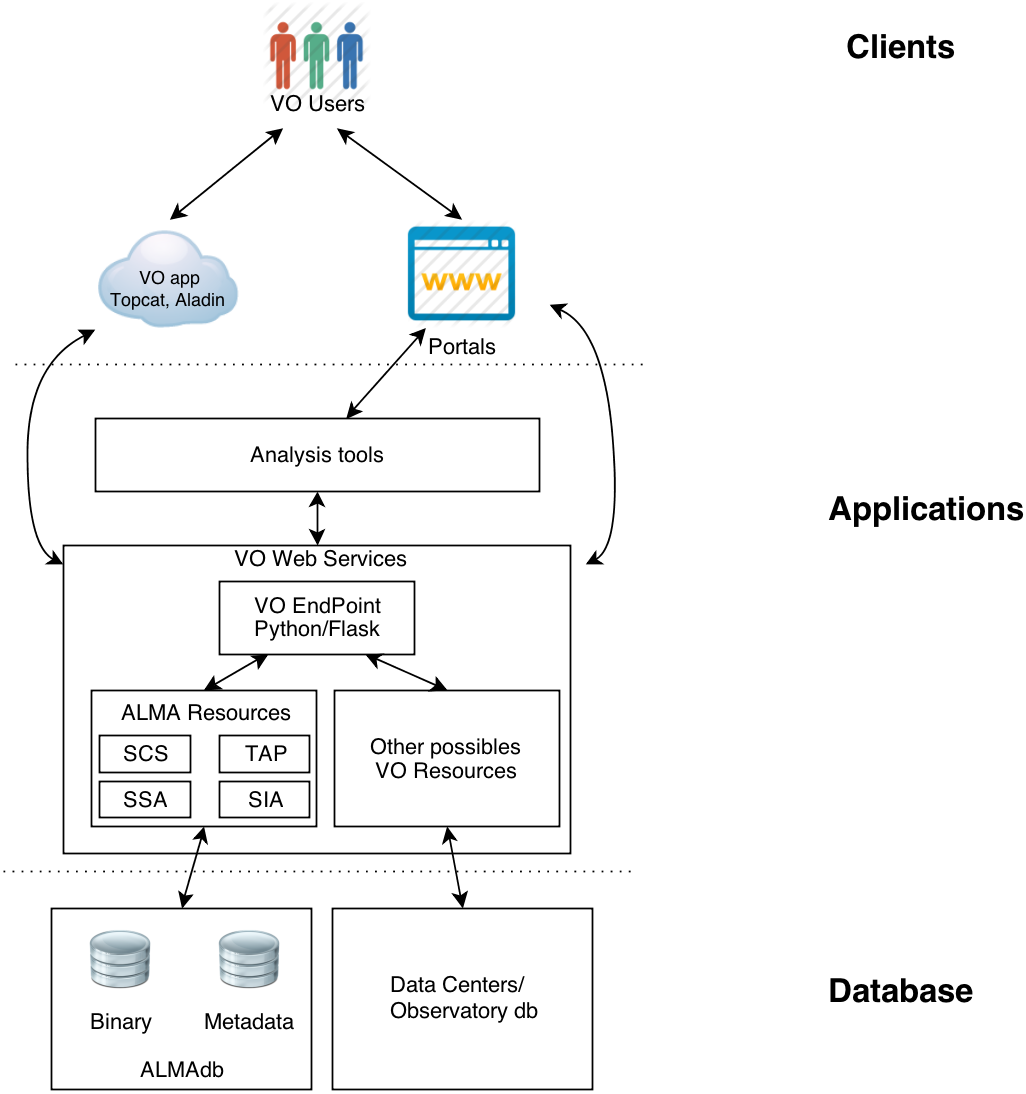
\includegraphics[width=0.6\textwidth]{img/chivo_capas.png}
        \caption{Arquitectura ChiVO - Tres capas.}
    \end{center}
\end{figure}

\subsection{Capa de Datos}
En esa capa residen los datos y es la encargada de organizar estos en una
estructura apropiada. Se implementó una base de datos relacional usando el
motor de base de datos postgresql \cite{psql} y el modelo de datos a usar es
ObsCore \cite{obscore}.

IVOA recomienda usar el modelo de datos ObsCore como base para su
interoperabilidad, definiendo columnas y tipos de datos conocidos de tal manera
que sea sencillo acceder y descrubrir información dentro de la base de datos.
Por otro lado todos los toolkits estudiados que soportan los Data Access Layer
en IVOA usan una función de postgresql llamada pgSphere \cite{pgsphere}. Estas
fueron las consideraciones para elegir dichas tecnologías.

Como los datos públicos del ciclo 0 de ALMA estarán todos disponibles en Abril
del 2014, en este prototipo se probó la interacción entre la capa de datos con
aplicación con datos de prueba. Una vez que todos estos datos estén disponibles
se poblará con datos reales la base de datos.

\subsection{Capa de Aplicación}
En la capa de aplicación están los programas que procesan las consultas de
forma de interactuar entre la capa de datos y usuarios. Para estos efectos se
creará en Web Service VO compliant.

En particular para este proyecto, según los requerimientos de la plataforma es
necesario configurar un recurso compatible con tecnologías de observatorio
virtual, y que permitan realizar 4 tipos de consultas basándose en los
protocolos: Simple Cone Search (SCS) \cite{scs}, Table Access Protocol (TAP)
\cite{tap}, Simple Spectral Access (SSA) \cite{ssa}, Simple Image Access (SIA)
\cite{sia}. Estos protocolos de comunicación establecen parámetros y tipos de
consultas HTTP básicas y opcionales para hacer acceder al sistema de datos.

Como es muy posible que más adelante se incluyan nuevos recursos para el
observatorio virtual (datos), es necesario generar una abstracción entre los
posibles clientes y todos estos recursos, el cual lo manejará un endpoint de
datos. Este endpoint además crea un marco para poder extender nuevas
funcionalidades para el sitio web, como por ejemplo, usuarios, seguridad,
caché, etc.

Para este prototipo se utilizó para configurar el ALMA Resources la herramienta
DaCHS \cite{dachs} desarrollada por el observatorio virtual Alemán, y para el
endpoint se usará la biblioteca de python/Flask \cite{flask}.

\subsection{Capa de Usuarios}
Esta capa es la que se le presenta finalmente al usuario y está destinada a
facilitar la comunicación entre el usuario y el sistema de datos. En esta capa
el usuario rellena información respecto a la consulta que quiere realizar,
usando 5 formularios posibles: 1 por cada protocolo de acceso, y un formulario
avanzado. Una vez que el usuario define su consulta el sistema le arroja los
objetos u observaciones candidatos de tal manera que pueda elegir cuales
descargar y usar de forma local. Para este entregable por ser prototipo se
implementaron los 4 forumarios para cada protocolo.

Esta capa se comunica directamente con el endpoint de datos mediante consultas
HTTP GET y POST, y el endpoint le retorna una tabla resultante de la consulta
en formato VOTable \cite{votable}. Este archivo mediante la herramienta VOview
\cite{voview} se muestra al usuario como tabla de datos.  Para este prototipo
se desarrolló un sitio web usando Ruby on Rails \cite{ror}.

\subsection{Descripción web service e integración}
Existe cierta secuencialidad en la interacción de un usuario con el sistema la que a grandes rasgos es:
\begin{enumerate}
	\item El usuario entra al sitio web e ingresa una consulta para obtener ciertos datos.
	\item El portal web hace hace una consulta al endpoint y queda esperando la respuesta.
	\item El endpoint recibe esta consulta, la valida, y la envía a DaCHS.
	\item Dachs ejecuta la consulta y recibe los datos los cuales deben llegar al usuario.
\end{enumerate}

Dentro de esta interacción es importante rescatar algunos aspectos de
escalabilidad (no implementados en el prototipo):
\begin{itemize}
	\item DaCHS y base de datos: estos componentes son relativamente
independiente, es decir, la aplicación DaCHS puede estar funcionando en
servidores distintos a la base de datos que se configuró (se puede configurar
un cluster de psql).
	\item Asincrono: cuando N usuarios ejecuten consultas de datos al mismo
tiempo, el endpoint recibirá también N consultas (N instancias) y lo mismo para
DaCHS, por lo que puede existir problema de eficiencia en este punto. Para
ello, se propone configurar más de un DaCHS, con cierta cantidad de base de
datos. La nueva tarea del endpoint será realizar un balance de carga entre los
servidores DaCHS antes de enviar la respectiva consulta. Esto asegura mayor
eficiencia, pero además se genera mayor necesidad de recursos computacionales.
	\item El punto anterior expone una necesidad opcional de tener una cola
opcional de tareas que sea manejado por algún servidor de mensajería (MQ
Server).
	\item Como el endpoint recibirá consultas para buscar datos y además
recibirá peticiones de descarga, se propone implementar un caché para alivianar
la carga de DaCHS y así aumentar la eficiencia del sistema.
\end{itemize}

\vspace{1.0cm}
\begin{figure}[h!t]
    \begin{center}
        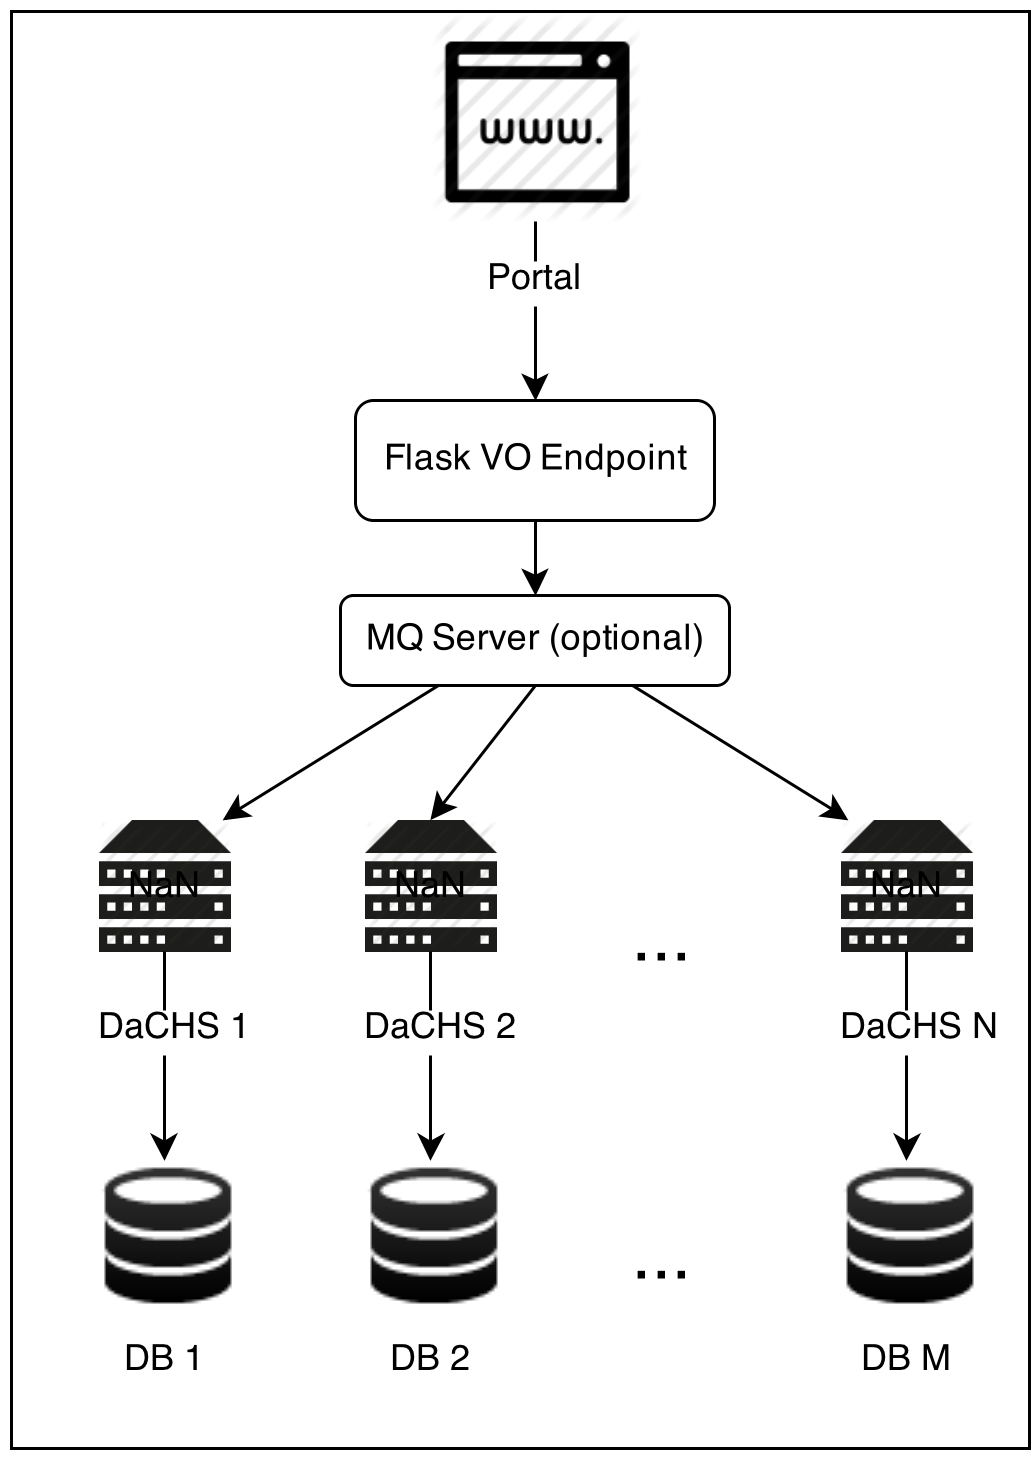
\includegraphics[width=0.4\textwidth]{img/interaccion.png}
        \caption{Arquitectura ChiVO - Interacción del servicio.}
    \end{center}
\end{figure}


\newpage
\thispagestyle{empty}
\addcontentsline{toc}{section}{Bibliografía}

\nocite{*}
\bibliographystyle{plain}
\bibliography{report}

\end{document}
